\documentclass{article}

% if you need to pass options to natbib, use, e.g.:
 \PassOptionsToPackage{numbers, compress}{natbib}
% before loading nips_2017
%
% to avoid loading the natbib package, add option nonatbib:
% \usepackage[nonatbib]{nips_2017}

% Keep final for now to remove annoying line numbers.
%\usepackage[final]{nips_2017}
% Keep final for now to remove annoying line numbers.


% to compile a camera-ready version, add the [final] option, e.g.:
\usepackage[final]{nips_2017}

\usepackage[utf8]{inputenc} % allow utf-8 input
\usepackage[T1]{fontenc}    % use 8-bit T1 fonts
\usepackage{hyperref}       % hyperlinks
\usepackage{url}            % simple URL typesetting
\usepackage{booktabs}       % professional-quality tables
\usepackage{amsfonts}       % blackboard math symbols
\usepackage{amsmath}
\usepackage{nicefrac}       % compact symbols for 1/2, etc.
\usepackage{microtype}      % microtypography
\usepackage{subfiles}
\usepackage{xcolor}
\usepackage{multirow}
\usepackage{enumerate}
\usepackage{subfiles}
\usepackage{multirow}
\usepackage{graphicx}
\usepackage{subfiles}
\usepackage{xeCJK}
\setCJKmainfont{SimSun}


% % Custom Commands:
% \newcommand\blfootnote[1]{%
%   \begingroup
%   \renewcommand\thefootnote{}\footnote{#1}%
%   \addtocounter{footnote}{-1}%
%   \endgroup
% }

\newcommand\todo[1]{\textcolor{red}{[[#1]]}}
\newcommand\mc[1]{\mathcal{#1}}
\newcommand*\samethanks[1][\value{footnote}]{\footnotemark[#1]}
%keys for memory and values. Can be changed if needed
\newcommand{\kq}{q}
\newcommand{\km}{k}
\newcommand{\vq}{o}
\newcommand{\vm}{m}
\newcommand{\Wkq}{W_q}
\newcommand{\Wkm}{W_k}
\newcommand{\Wvq}{W_o}
\newcommand{\Wvm}{W_m}
\newcommand{\dmodel}{d_{\text{model}}}
\newcommand{\dffn}{d_{\text{ffn}}}
\newcommand{\dff}{d_{\text{ff}}}
\newcommand{\mbf}[1]{\mathbf{#1}}
%\newcommand{\kq}{{q}_k}
%\newcommand{\km}{{m}_k}
%\newcommand{\vq}{{q}_v}
%\newcommand{\vm}{{m}_v}
%\newcommand{\Wkq}{{W_q}_k}
%\newcommand{\Wkm}{{W_m}_k}
%\newcommand{\Wvq}{{W_q}_v}
%\newcommand{\Wvm}{{W_m}_v}
\newcommand\concat[3]{\left[#1 \parallel_#3 #2\right]}

\title{Attention Is All You Need}

% The \author macro works with any number of authors. There are two
% commands used to separate the names and addresses of multiple
% authors: \And and \AND.
%
% Using \And between authors leaves it to LaTeX to determine where to
% break the lines. Using \AND forces a line break at that point. So,
% if LaTeX puts 3 of 4 authors names on the first line, and the last
% on the second line, try using \AND instead of \And before the third
% author name.
\author{
  \AND
  Ashish Vaswani\thanks{贡献相等。作者列表顺序随机。Jakob 提出用自注意力机制替换 RNN 并开始评估这一想法。
Ashish 与 Illia 设计并实现了第一个 Transformer 模型,并参与了这项工作的各个方面。Noam 提出了缩放点积注意力、多头注意力以及无参数的位置表示,并成为几乎参与每个细节的另一位成员。Niki 在我们原始的代码库和 tensor2tensor 中设计、实现、调整和评估了无数模型变体。Llion 也尝试了新颖的模型变体,负责我们最初的代码库、高效推理和可视化。Lukasz 和 Aidan 花费了无数个漫长的日子设计各个部分并实现 tensor2tensor,取代了我们早期的代码库,极大地改善了结果并加速了我们的研究。
}\\
  Google Brain\\
  \texttt{avaswani@google.com}\\
  \And
  Noam Shazeer\footnotemark[1]\\
  Google Brain\\
  \texttt{noam@google.com}\\
  \And
  Niki Parmar\footnotemark[1]\\
  Google Research\\
  \texttt{nikip@google.com}\\
  \And
  Jakob Uszkoreit\footnotemark[1]\\
  Google Research\\
  \texttt{usz@google.com}\\
  \And
  Llion Jones\footnotemark[1]\\
  Google Research\\
  \texttt{llion@google.com}\\
  \And
  Aidan N. Gomez\footnotemark[1] \hspace{1.7mm}\thanks{工作完成于 Google Brain 期间。}\\
  University of Toronto\\
  \texttt{aidan@cs.toronto.edu}
  \And
  {\L}ukasz Kaiser\footnotemark[1]\\
  Google Brain\\
  \texttt{lukaszkaiser@google.com}\\
  \And
  Illia Polosukhin\footnotemark[1]\hspace{1.7mm} \thanks{工作完成于 Google Research 期间。}\\
  \texttt{illia.polosukhin@gmail.com}\\
}

\begin{document}
\begin{center}
    \color{red}
    \large 在提供适当署名的前提下,Google 特此授予仅为新闻或学术作品复制本文中表格和图形的许可。
\end{center}

\maketitle

\begin{abstract}
主流的序列转导模型基于包含编码器和解码器的复杂循环或卷积神经网络。性能最佳的模型还通过注意力机制连接编码器和解码器。我们提出了一种新的简单网络架构——Transformer,它完全基于注意力机制,完全摒弃了循环和卷积。在两个机器翻译任务上的实验表明,这些模型在质量上更优,同时更具可并行性,并且需要的训练时间显著减少。我们的模型在 WMT 2014 英语-德语翻译任务上取得了 28.4 的 BLEU 分数,比现有最佳结果(包括集成模型)提高了超过 2 个 BLEU 分数。在 WMT 2014 英语-法语翻译任务上,我们的模型在 8 个 GPU 上训练 3.5 天后,建立了新的单模型最先进 BLEU 分数 41.8,这仅是文献中最佳模型训练成本的一小部分。我们通过将 Transformer 成功应用于英语成分句法分析(无论训练数据量大小),表明其能很好地推广到其他任务。
% \blfootnote{代码可在 \url{链接} 获取}

%TODO(noam): update results for new models.

%llion@: FAIR's paper seems to concentrate solely on the convolutional aspect of their model and have the attention as an after thought almost, this gives us a good opportunity to differentiate ourselves from their paper.

%We are simpler in a number of ways and should have the simplicity as a big selling point:
%\begin{itemize}
%\item No convolutions
%\item No need for such careful initializations and %normalization.
%\item Simpler non-lineararities, they use the gated linear %units.
%\item Less layers?
%\end{itemize}
%One thing we do more is that we have self attention.
%Another selling point is the increased interpretability as %shown with the visualizations. Which comes from the %simplicity and use of only attentions.
\end{abstract}

\section{引言}

循环神经网络,尤其是长短期记忆网络\citep{hochreiter1997}和门控循环单元网络\citep{gruEval14},已被牢固确立为序列建模和转换问题(如语言建模和机器翻译)中最先进的方法\citep{sutskever14, bahdanau2014neural, cho2014learning}。此后,许多努力不断推动循环语言模型和编码器-解码器架构的边界\citep{wu2016google,luong2015effective,jozefowicz2016exploring}。

循环模型通常沿着输入和输出序列的符号位置分解计算。将位置与计算时间步骤对齐,它们生成一系列隐藏状态$h_t$,作为前一个隐藏状态$h_{t-1}$和位置$t$的输入的函数。这种固有的顺序性质阻止了训练示例内的并行化,这在序列长度较长时变得关键,因为内存限制限制了示例间的批处理。

%\marginpar{不确定这里的内存限制是否易于理解}
近期工作通过分解技巧\citep{Kuchaiev2017Factorization}和条件计算\citep{shazeer2017outrageously}实现了计算效率的显著提升,同时在后者的情况下还提高了模型性能。然而,顺序计算的基本约束仍然存在。

%\marginpar{@all: 有工作分析注意力在seq2seq模型中的实际作用,但一时找不到}

注意力机制已成为各种任务中引人注目的序列建模和转换模型不可或缺的组成部分,允许对依赖关系进行建模而无视其在输入或输出序列中的距离\citep{bahdanau2014neural, structuredAttentionNetworks}。但在除少数情况外\citep{decomposableAttnModel},此类注意力机制与循环网络结合使用。

%\marginpar{不确定"跨位置通信"是否无需解释即可理解}
%\marginpar{插入达到SOTA最早模型的精确训练时间和统计,或许甚至是单GPU模型?}

在这项工作中,我们提出了Transformer,一种避免循环并完全依赖注意力机制来绘制输入和输出之间全局依赖关系的模型架构。Transformer允许显著更多的并行化,并且在八个P100 GPU上训练仅十二小时后即可达到翻译质量的新 state of the art。
%\marginpar{你移除了恒定重复次数部分。我写它是为了明确模型不仅执行一次注意力,同时也不是循环的。我认为尽早传达这一点可能很重要。}

% 只是一个带引用的标准段落,重写。
%在\citep{sutskever14}、\citep{bahdanau2014neural}和\citep{cho2014learning}的开创性论文之后,循环模型已成为序列建模和序列到序列转换的主导解决方案。许多努力如\citep{wu2016google,luong2015effective,jozefowicz2016exploring}利用循环序列模型推动了机器翻译和语言建模的边界。最近的工作\citep{shazeer2017outrageously}将条件计算的力量与序列模型结合,训练了用于机器翻译的非常大型的模型,以较低计算成本推高了SOTA。循环模型为每个计算时间步骤t计算隐藏状态向量h_t。h_t是时间t的输入和前一隐藏状态h_t的函数。这种对前一隐藏状态的依赖使循环模型难以同时处理多个输入,其时间复杂性是输入和输出长度的线性函数,无论是在训练还是推理期间。[我想在这里说的是,尽管在解码时这没问题,但在训练时,我们同时有输入和输出,这种线性性质不允许RNN同时处理所有输入和输出,并且尚未用于网络规模的数据集。我们拥有的最大数据集是什么?谈论Nvidia和其他公司加速工作的努力,以及其他缓解此问题但仍受其计算性质限制的努力]。引言其余部分:如果你能基于实际输入和输出构建状态,那么你就可以一次性构建它们。这已成为许多近期有希望的努力的基础,如bytenet、facenet(也在这里讨论quasi rnn)。现在我们讨论注意力!!与细胞架构如长短期记忆(LSTM)\citep{hochreiter1997}和门控循环单元(GRUs)\citep{cho2014learning}一起,注意力已成为成功序列模型中的重要组成部分,尤其是在机器翻译中。近年来,机器翻译中许多(如果不是全部)state-of-the-art(SOTA)结果都是通过基于注意力的序列模型实现的\citep{wu2016google,luong2015effective,jozefowicz2016exploring}。谈论neon工作中如何通过自注意力玩转注意力!然后谈论我们的工作。


\section{背景}

减少序列计算的目标同样构成了扩展神经GPU\citep{extendedngpu}、ByteNet\citep{NalBytenet2017}和ConvS2S\citep{JonasFaceNet2017}的基础,这些模型均使用卷积神经网络作为基本构建模块,并行计算所有输入和输出位置的隐藏表示。在这些模型中,关联两个任意输入或输出位置信号所需的操作次数随位置间距离的增长而增加:ConvS2S为线性增长,ByteNet为对数增长。这使得学习远距离位置之间的依赖关系变得更加困难\citep{hochreiter2001gradient}。在Transformer中,这一操作次数被减少到一个常数级别,尽管这是以降低有效分辨率为代价的(因为对注意力加权的位置进行了平均),我们通过第~\ref{sec:attention}节所述的多头注意力机制来抵消这种影响。

自注意力(Self-attention),有时也称为内部注意力(intra-attention),是一种关联单个序列中不同位置的注意力机制,目的是计算该序列的表示。自注意力已成功应用于多种任务,包括阅读理解、抽象摘要、文本蕴含学习以及任务无关的句子表示学习\citep{cheng2016long, decomposableAttnModel, paulus2017deep, lin2017structured}。

端到端记忆网络基于循环注意力机制而非序列对齐的循环,并已被证明在简单语言问答和语言建模任务上表现良好\citep{sukhbaatar2015}。

然而,据我们所知,Transformer是第一个完全依赖自注意力来计算其输入和输出表示的转换模型,而没有使用序列对齐的RNN或卷积。在接下来的章节中,我们将描述Transformer的架构,解释自注意力的动机,并讨论其相对于\citep{neural_gpu, NalBytenet2017}和\citep{JonasFaceNet2017}等模型的优势。


%\citep{JonasFaceNet2017} 报告了在英语-德语、英语-法语和英语-罗马尼亚语机器翻译任务上达到的新SOTA结果。

%例如,在机器翻译中,我们必须同时从输入词和先前的输出词中提取信息,以准确地翻译一个输出词。注意力层\citep{bahdanau2014neural}能够以较低的计算成本连接非常多的位置,这使其成为具有竞争力的机器翻译循环模型中的关键组成部分。

%那么一个很自然的问题是:“我们能否用注意力来替代循环?”。这样的模型将兼具注意力的计算效率和跨位置通信的能力。在这项工作中,我们证明了纯注意力模型在机器翻译上表现非常出色,在英德和英法翻译上取得了新的SOTA结果,并且可以在xyz架构上在$2$天内完成训练。

%在\citep{sutskever14, bahdanau2014neural, cho2014learning}提出的开创性模型之后,循环模型已成为序列建模和序列到序列转换任务的主导解决方案。许多努力,例如\citep{wu2016google,luong2015effective,jozefowicz2016exploring},通过循环编码器-解码器和循环语言模型不断推进机器翻译和语言建模的边界。最近的工作\citep{shazeer2017outrageously}成功地将条件计算的能力与序列模型相结合,以更低的计算成本训练用于机器翻译的超大模型,并推动了SOTA水平。

%循环模型为计算的每个时间步$t$计算一个隐藏状态向量$h_t$。$h_t$是时间$t$的输入和前一隐藏状态$h_t$的函数。这种对前一隐藏状态的依赖阻止了所有时间步的同时处理,反而需要一长串的顺序操作。在实践中,这导致计算效率大大降低,因为在现代计算硬件上,对大批量数据的单次操作远比对小批量的多次操作快得多。序列越长,问题越严重。尽管顺序计算在推理时并非严重瓶颈,因为自回归地生成每个输出都需要所有先前的输出,但无法同时计算所有输出位置的分数阻碍了我们在大型数据集上快速训练模型。尽管像\citep{Kuchaiev2017Factorization}这样令人印象深刻的工作能够通过因子化技巧显著加速LSTM的训练,我们仍然受限于对序列长度的线性依赖。

%如果模型能够仅使用输入和输出来计算每个时间步的隐藏状态,那么在训练期间它将摆脱对前一时间步结果的依赖。这一思路是近期诸如马尔可夫神经GPU\citep{neural_gpu}、ByteNet\citep{NalBytenet2017}和ConvS2S\citep{JonasFaceNet2017}等工作的基础,这些工作都使用卷积神经网络作为构建块来同时计算所有时间步的隐藏表示,从而实现了$O(1)$的顺序时间复杂度。\citep{JonasFaceNet2017}报告了在英语-德语、英语-法语和英语-罗马尼亚语机器翻译任务上达到的新SOTA结果。

%精确序列预测的一个关键组成部分是对跨位置通信的建模。例如,在机器翻译中,我们必须同时从输入词和先前的输出词中提取信息,以准确地翻译一个输出词。注意力层\citep{bahdanau2014neural}能够以较低的计算成本(同样具有$O(1)$的顺序时间复杂度)连接非常多的位置,这使其成为机器翻译中循环编码器-解码器架构的关键组成部分。那么一个很自然的问题是:“我们能否用注意力来替代循环?”。这样的模型将兼具注意力的计算效率和跨位置通信的能力。在这项工作中,我们证明了纯注意力模型在机器翻译上表现非常出色,在英德和英法翻译上取得了新的SOTA结果,并且可以在xyz架构上在$2$天内完成训练。



%注意:Facebook的模型在这方面并不比RNN更好,因为它需要与所需通信距离成比例的层数。ByteNet更有前途,因为它需要层数是对数级的(ByteNet有SOTA结果吗)?

%注意:注意力层能够以$O(1)$顺序操作的低计算成本连接非常多的位置。这就是为什么编码器-解码器注意力在序列到序列模型中如此成功的原因。那么,很自然地,也可以使用注意力来连接同一序列的时间步。

%注意:我不会说长序列在推理时不是问题。如果我们能在没有长序列的情况下进行推理,那就太好了。我们可以稍后说明,虽然我们的训练图是恒定深度的,但由于模型的自回归特性,我们的模型在推理时解码器部分仍然需要顺序操作。

%\begin{table}[h!]
%\caption{当序列长度小于通道深度时,注意力模型对于跨位置通信是相当高效的。$n$代表序列长度,$d$代表通道深度。}
%\label{tab:op_complexities}
%\begin{center}
%\vspace{-5pt}
%\scalebox{0.75}{

%\begin{tabular}{l|c|c|c}
%\hline \hline
%层类型 & 感受野 & 计算复杂度 & 顺序操作数 \\
%\hline
%逐点前馈网络 & $1$ & $O(n \cdot d^2)$ & $O(1)$ \\
%\hline
%循环层 & $n$ & $O(n \cdot d^2)$ & $O(n)$ \\
%\hline
%卷积层 & $r$ & $O(r \cdot n \cdot d^2)$ & $O(1)$ \\
%\hline
%卷积层(可分离)& $r$ & $O(r \cdot n \cdot d + n \cdot d^2)$ & $O(1)$ \\
%\hline
%注意力层 & $r$ & $O(r \cdot n \cdot d)$ & $O(1)$ \\
%\hline \hline
%\end{tabular}
%}
%\end{center}
%\end{table}


\section{模型架构}
\begin{figure}
  \centering
  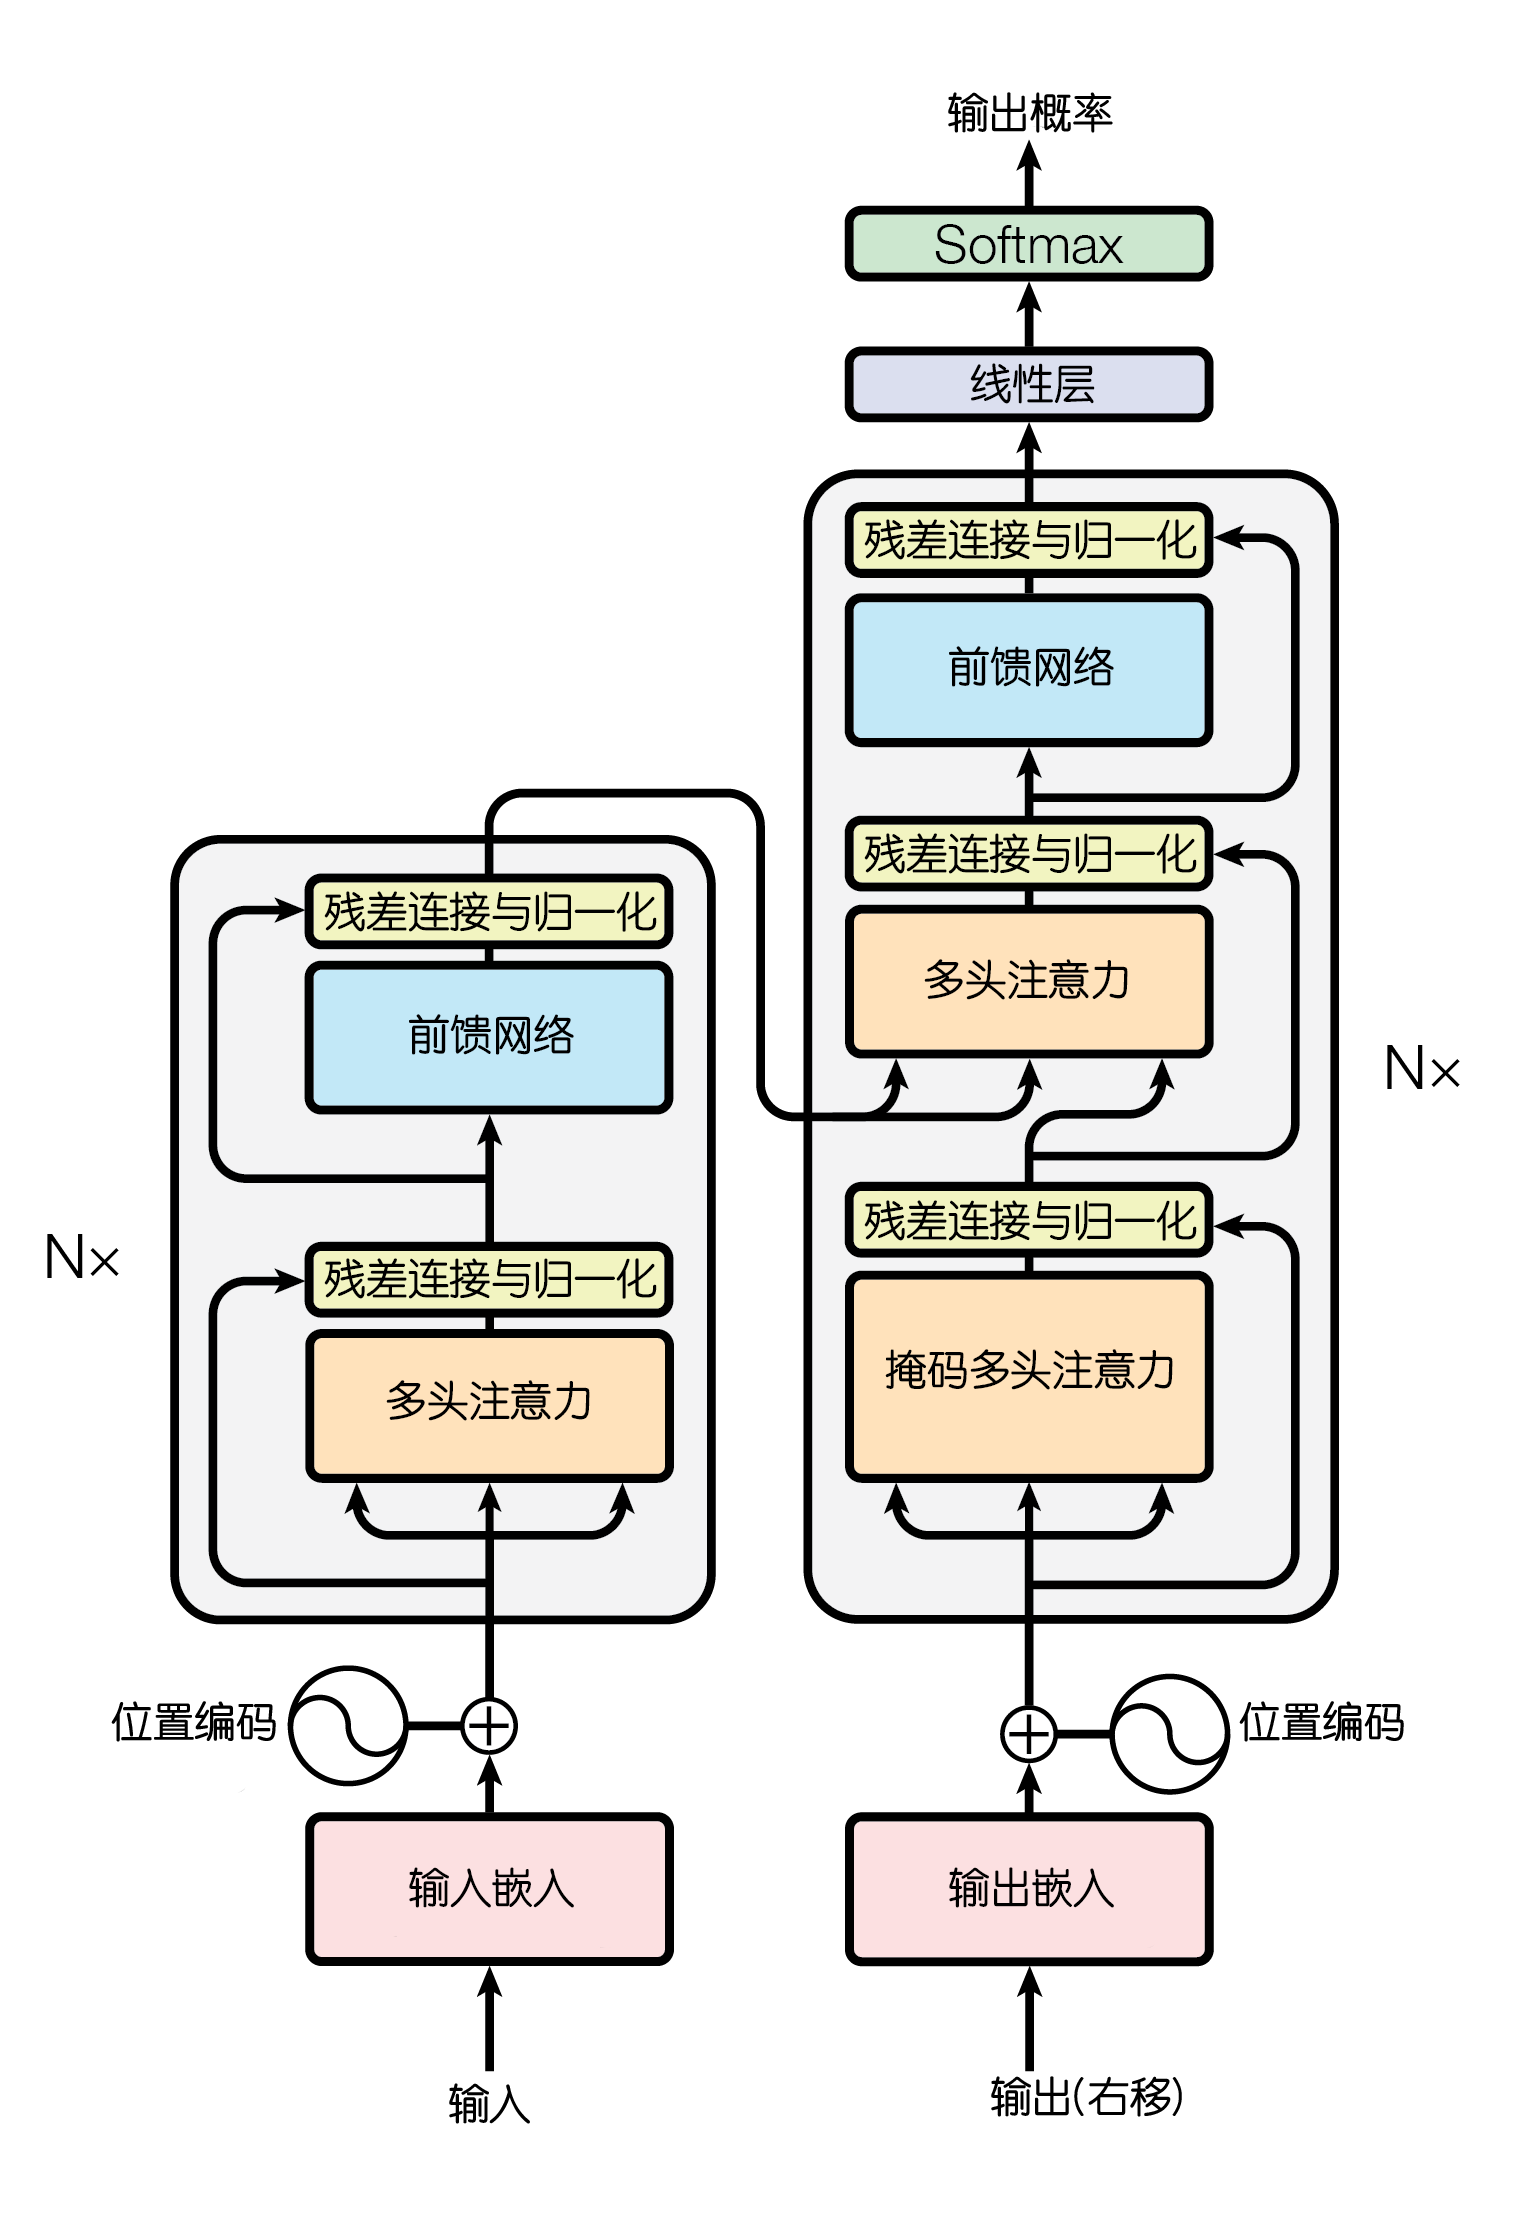
\includegraphics[scale=0.6]{Figures/ModalNet-21}
  \caption{Transformer 模型架构。}
  \label{fig:model-arch}
\end{figure}

% 尽管我们模型的主要组成部分是注意力,
% 我们的模型保持了编码器-解码器结构,这种结构在许多所谓的序列到序列模型中很常见 \citep{bahdanau2014neural,sutskever14}。与所有此类架构一样,编码器计算输入序列的表示,解码器消耗这些表示以及输出标记,以自回归的方式产生输出序列。传统上,编码器和解码器包含循环或卷积层堆叠,而我们的编码器和解码器堆叠由注意力层和逐位置前馈层组成(图~\ref{fig:model-arch})。以下章节详细描述了整体架构和这些特定组件。

大多数具有竞争力的神经序列转导模型都具有编码器-解码器结构 \citep{cho2014learning,bahdanau2014neural,sutskever14}。这里,编码器将符号表示的输入序列 $(x_1, ..., x_n)$ 映射到连续表示的序列 $\mathbf{z} = (z_1, ..., z_n)$。给定 $\mathbf{z}$,解码器然后一次一个元素地生成符号的输出序列 $(y_1,...,y_m)$。在每一步,模型是自回归的 \citep{graves2013generating},在生成下一个符号时消耗先前生成的符号作为额外输入。

Transformer 遵循这种整体架构,对编码器和解码器使用堆叠的自注意力和逐点全连接层,分别如图~\ref{fig:model-arch} 的左右半部分所示。

\subsection{编码器和解码器堆叠}

\paragraph{编码器:}编码器由 $N=6$ 个相同层堆叠而成。每层有两个子层。第一个是多头自注意力机制,第二个是简单的逐位置全连接前馈网络。我们在每个子层周围使用残差连接 \citep{he2016deep},然后进行层归一化 \cite{layernorm2016}。也就是说,每个子层的输出是 $\mathrm{LayerNorm}(x + \mathrm{Sublayer}(x))$,其中 $\mathrm{Sublayer}(x)$ 是子层本身实现的函数。为了促进这些残差连接,模型中的所有子层以及嵌入层都产生维度 $\dmodel=512$ 的输出。

\paragraph{解码器:}解码器也由 $N=6$ 个相同层堆叠而成。除了每个编码器层中的两个子层外,解码器插入第三个子层,该子层对编码器堆叠的输出执行多头注意力。与编码器类似,我们在每个子层周围使用残差连接,然后进行层归一化。我们还修改了解码器堆叠中的自注意力子层,以防止位置关注到后续位置。这种掩码结合输出嵌入偏移一个位置的事实,确保对位置 $i$ 的预测只能依赖于位置小于 $i$ 的已知输出。

% 在我们的模型(图~\ref{fig:model-arch})中,编码器和解码器由交替的自注意力层(用于跨位置通信)和逐位置前馈层(用于就地计算)堆叠而成。此外,解码器堆叠包含编码器-解码器注意力层。由于注意力对词之间的距离不可知,我们的模型需要向编码器和解码器输入添加“位置编码”。以下章节详细描述所有这些组件。

\subsection{注意力} \label{sec:attention}
注意力函数可以描述为将查询和一组键值对映射到输出,其中查询、键、值和输出都是向量。输出计算为值的加权和,其中分配给每个值的权重通过查询与相应键的兼容性函数计算。

\subsubsection{缩放点积注意力} \label{sec:scaled-dot-prod}

% \begin{figure}
%   \centering
%   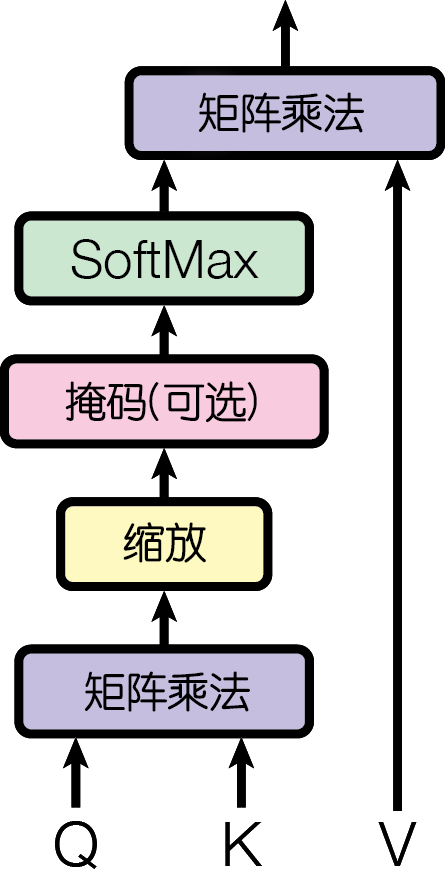
\includegraphics[scale=0.6]{Figures/ModalNet-19}
%   \caption{缩放点积注意力。}
%   \label{fig:multi-head-att}
% \end{figure}

我们将我们的特定注意力称为“缩放点积注意力”(图~\ref{fig:multi-head-att})。输入由维度 $d_k$ 的查询和键,以及维度 $d_v$ 的值组成。我们计算查询与所有键的点积,每个除以 $\sqrt{d_k}$,然后应用 softmax 函数来获得值的权重。

在实践中,我们同时计算一组查询的注意力函数,将它们打包成矩阵 $Q$。键和值也打包成矩阵 $K$ 和 $V$。我们计算输出矩阵为:

\begin{equation}
   \mathrm{Attention}(Q, K, V) = \mathrm{softmax}(\frac{QK^T}{\sqrt{d_k}})V
\end{equation}

两种最常用的注意力函数是加性注意力 \citep{bahdanau2014neural} 和点积(乘法)注意力。点积注意力与我们的算法相同,除了缩放因子 $\frac{1}{\sqrt{d_k}}$。加性注意力使用具有单个隐藏层的前馈网络计算兼容性函数。虽然两者在理论复杂度上相似,但点积注意力在实践中更快且更节省空间,因为它可以使用高度优化的矩阵乘法代码实现。

% 我们将点积缩放 $1/\sqrt{d_k}$ 以限制点积的幅度,这在实践中效果很好。否则,我们发现应用 softmax 通常会导致权重非常接近 0 或 1,从而产生极小的梯度。

% 已在后续章节描述
% 当用作解码器自注意力的一部分时,在 softmax 之前应用可选的掩码函数以防止位置关注到后续位置。该掩码简单地将所有非法连接(下三角外部)对应的 logits 设置为 $-\infty$。

%\paragraph{与加性注意力的比较:} 我们选择点积注意力而非加性注意力 \citep{bahdanau2014neural},因为它可以使用高度优化的矩阵乘法代码计算。这种优化对我们尤为重要,因为我们在模型中使用了许多注意力层。

虽然对于较小的 $d_k$ 值,两种机制表现相似,但对于较大的 $d_k$ 值,不加缩放的点积注意力不如加性注意力 \citep{DBLP:journals/corr/BritzGLL17}。我们怀疑对于较大的 $d_k$ 值,点积的幅度会变大,将 softmax 函数推入梯度极小的区域\footnote{为了说明点积为何变大,假设 $q$ 和 $k$ 的分量是均值为 $0$、方差为 $1$ 的独立随机变量。那么它们的点积 $q \cdot k = \sum_{i=1}^{d_k} q_ik_i$ 的均值为 $0$,方差为 $d_k$。}。为了抵消这种效应,我们将点积缩放 $\frac{1}{\sqrt{d_k}}$。

% 我们怀疑这是因为点积幅度变得过大,导致应用 softmax 函数后梯度无用。为了抵消这一点,我们将点积缩放 $1/\sqrt{d_k}$。

\subsubsection{多头注意力} \label{sec:multihead}

\begin{figure}
\begin{minipage}[t]{0.5\textwidth}
  \centering
  缩放点积注意力 \\
  \vspace{0.5cm}
  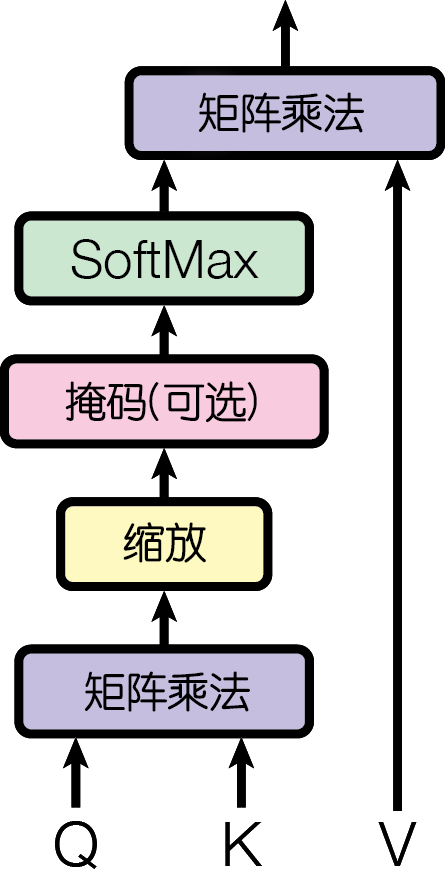
\includegraphics[scale=0.6]{Figures/ModalNet-19}
\end{minipage}
\begin{minipage}[t]{0.5\textwidth}
  \centering 
  多头注意力 \\
  \vspace{0.1cm}
  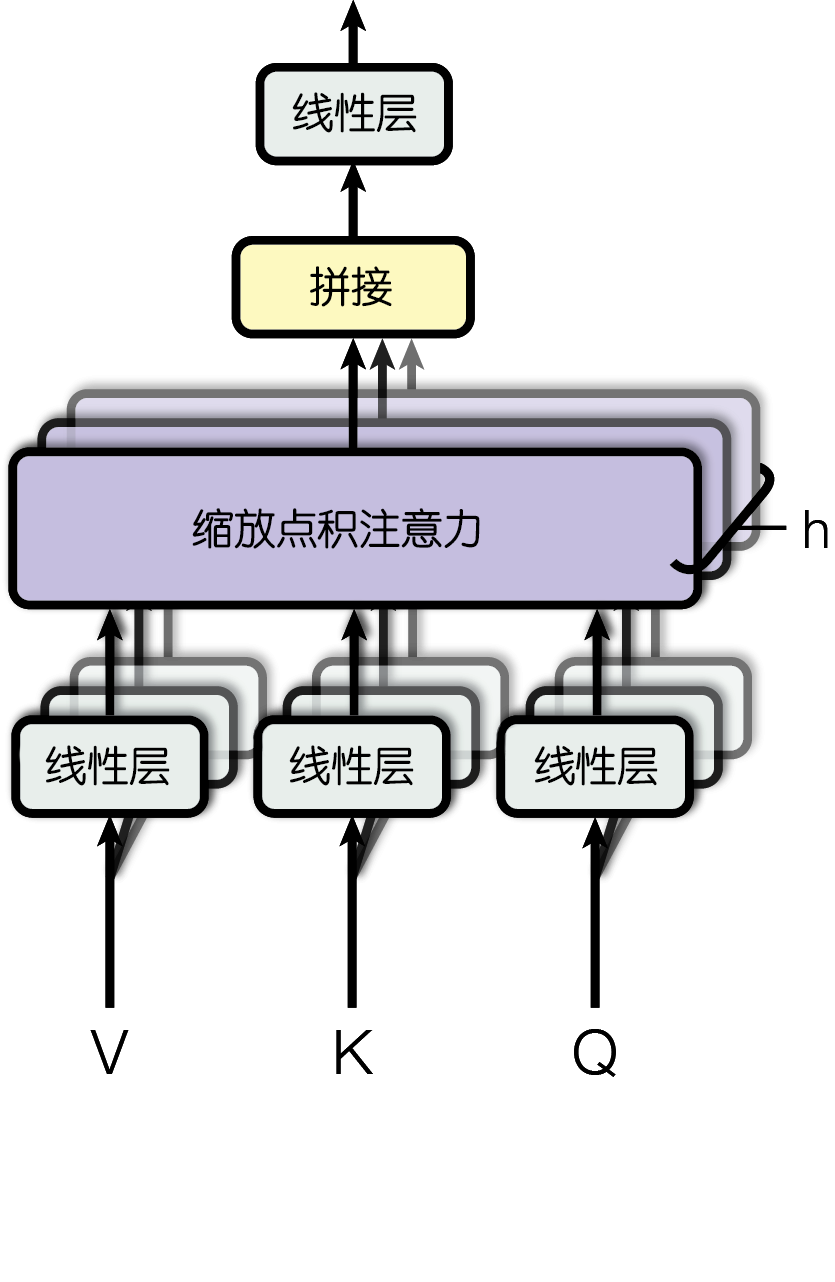
\includegraphics[scale=0.6]{Figures/ModalNet-20}  
\end{minipage}


  % \centering

  \caption{(左)缩放点积注意力。(右)多头注意力由几个并行运行的注意力层组成。}
  \label{fig:multi-head-att}
\end{figure}

我们发现,与使用 $\dmodel$ 维键、值和查询执行单个注意力函数相比,将查询、键和值用不同的学习线性投影线性投影 $h$ 次到 $d_k$、$d_k$ 和 $d_v$ 维度是有益的。
然后我们在这些投影版本的查询、键和值上并行执行注意力函数,产生 $d_v$ 维输出值。这些输出被连接并再次投影,得到最终值,如图~\ref{fig:multi-head-att} 所示。

多头注意力允许模型在不同位置联合关注来自不同表示子空间的信息。使用单个注意力头时,平均会抑制这一点。

\begin{align*}
    \mathrm{MultiHead}(Q, K, V) &= \mathrm{Concat}(\mathrm{head_1}, ..., \mathrm{head_h})W^O\\
%    \mathrm{where} \mathrm{head_i} &= \mathrm{Attention}(QW_Q_i^{\dmodel \times d_q}, KW_K_i^{\dmodel \times d_k}, VW^V_i^{\dmodel \times d_v})\\
    \text{其中}~\mathrm{head_i} &= \mathrm{Attention}(QW^Q_i, KW^K_i, VW^V_i)\\
\end{align*}

其中投影是参数矩阵 $W^Q_i \in \mathbb{R}^{\dmodel \times d_k}$, $W^K_i \in \mathbb{R}^{\dmodel \times d_k}$, $W^V_i \in \mathbb{R}^{\dmodel \times d_v}$ 和 $W^O \in \mathbb{R}^{hd_v \times \dmodel}$。

% 我们发现(且成本不更高)使用多个并行注意力层(每个层覆盖全部位置),其键、值和查询维度按比例降低更好。我们称之为“多头注意力”(图~\ref{fig:multi-head-att})。每个并行注意力层的键、值和查询通过对多头注意力的输入进行学习线性变换计算。我们在不同并行注意力层之间使用不同的线性变换。并行注意力层的输出被连接,然后通过最终的学习线性变换。

在这项工作中,我们使用 $h=8$ 个并行注意力层或头。对于每个头,我们使用 $d_k=d_v=\dmodel/h=64$。
由于每个头的维度减少,总计算成本与全维单头注意力相似。

\subsubsection{注意力在我们模型中的应用}

Transformer 在三个方面使用多头注意力:
\begin{itemize}
 \item 在“编码器-解码器注意力”层中,查询来自前一个解码器层,记忆键和值来自编码器的输出。这允许解码器中的每个位置关注输入序列中的所有位置。这模仿了序列到序列模型中的典型编码器-解码器注意力机制,例如 \citep{wu2016google, bahdanau2014neural,JonasFaceNet2017}。

 \item 编码器包含自注意力层。在自注意力层中,所有键、值和查询来自相同的地方,即编码器中前一层的输出。编码器中的每个位置可以关注编码器前一层中的所有位置。

 \item 类似地,解码器中的自注意力层允许解码器中的每个位置关注解码器中包括该位置在内的所有位置。我们需要防止解码器中的向左信息流以保持自回归特性。我们通过在 softmax 的输入中将所有对应非法连接的值掩码(设置为 $-\infty$)来实现这一点。见图~\ref{fig:multi-head-att}。

\end{itemize}

\subsection{逐位置前馈网络}\label{sec:ffn}

除了注意力子层外,编码器和解码器的每个层都包含一个全连接前馈网络,该网络分别且相同地应用于每个位置。这包括两个线性变换,中间有 ReLU 激活。

\begin{equation}
   \mathrm{FFN}(x)=\max(0, xW_1 + b_1) W_2 + b_2
\end{equation}

虽然线性变换在不同位置相同,但它们在层与层之间使用不同的参数。另一种描述方式是使用核大小为 1 的两个卷积。输入和输出的维度为 $\dmodel=512$,内层维度为 $d_{ff}=2048$。

% 在附录中,我们描述了逐位置前馈网络如何也可以被视为注意力的一种形式。

%来自 Jakob:模型关联两个任意输入或输出位置信号所需的操作数随输入或输出中位置之间的距离增长,对于 ConvS2S 线性增长,对于 ByteNet 对数增长,使得学习这些位置之间的依赖关系更加困难 \citep{hochreiter2001gradient}。在 Transformer 中,这减少为常数操作数,尽管代价是由于平均注意力加权位置导致的有效分辨率降低,我们旨在通过多头注意力抵消这种效应。

%图~\ref{fig:simple-att} 展示了一个简单的注意力函数 $A$,具有单个头,构成我们多头注意力的基础。$A$ 接受查询键向量 $\kq$、记忆键矩阵 $\km$ 和记忆值矩阵 $\vm$,并产生查询值向量 $\vq$ 作为
%\begin{equation*} \label{eq:attention}
%    A(\kq, \km, \vm) = {\vm}^T (Softmax(\km \kq).
%\end{equation*}
%在调用注意力函数之前,我们使用学习矩阵 ${\Wkq \text{,} \, \Wkm}$ 和 ${\Wvm}$ 线性变换 $\kq,\,\km$ 和 $\vm$,并在将其传递给前馈层之前使用 $\Wvq$ 变换输出查询。每个注意力层有自己的一组变换矩阵,这些矩阵在所有查询位置共享。$A$ 在每个查询位置并行应用,并作为矩阵乘法的批处理高效实现。自注意力和编码器-解码器注意力层使用 $A$,但参数不同。例如,在编码器自注意力中,编码器层 $i$ 中的查询关注编码器层 $i-1$ 中的记忆。为确保解码器自注意力层不查看未来词,我们为查询位置 $l$ 将位置 $j+1$ 到查询长度的 logits 添加 $- \inf$。

%在简单注意力中,查询值是记忆值的加权组合,其中注意力权重和为 1。尽管该函数在实践中表现良好,但注意力权重的约束可能限制从记忆到查询的信息流,因为查询不能同时关注多个记忆位置,这在翻译长序列时可能是可取的。\marginpar{@usz,你能想到一个例子吗?} 我们通过在每个查询位置维护多个注意力头来补救,这些头并行关注所有记忆位置,每个注意力头 $h$ 有不同参数集。
%\marginpar{}

\subsection{嵌入和 Softmax}
与其他序列转导模型类似,我们使用学习嵌入将输入标记和输出标记转换为维度 $\dmodel$ 的向量。我们还使用通常的学习线性变换和 softmax 函数将解码器输出转换为预测的下一个标记概率。在我们的模型中,我们在两个嵌入层和 softmax 前线性变换之间共享相同的权重矩阵,类似于 \citep{press2016using}。在嵌入层中,我们将这些权重乘以 $\sqrt{\dmodel}$。

\subsection{位置编码}
由于我们的模型不包含循环和卷积,为了使模型利用序列的顺序,我们必须注入关于序列中标记的相对或绝对位置的信息。为此,我们在编码器和解码器堆叠的底部向输入嵌入添加“位置编码”。位置编码具有与嵌入相同的维度 $\dmodel$,以便两者可以相加。位置编码有许多选择,学习的和固定的 \citep{JonasFaceNet2017}。

在这项工作中,我们使用不同频率的正弦和余弦函数:

\begin{align*}
    PE_{(pos,2i)} = sin(pos / 10000^{2i/\dmodel}) \\
    PE_{(pos,2i+1)} = cos(pos / 10000^{2i/\dmodel})
\end{align*}

其中 $pos$ 是位置,$i$ 是维度。也就是说,位置编码的每个维度对应一个正弦曲线。波长形成从 $2\pi$ 到 $10000 \cdot 2\pi$ 的几何级数。我们选择这个函数是因为我们假设它允许模型轻松学习通过相对位置关注,因为对于任何固定偏移 $k$,$PE_{pos+k}$ 可以表示为 $PE_{pos}$ 的线性函数。

我们还尝试使用学习的位置嵌入 \citep{JonasFaceNet2017},发现两个版本产生几乎相同的结果(见表~\ref{tab:variations} 行 (E))。我们选择正弦版本,因为它可能允许模型外推到训练期间遇到的序列长度更长的序列。


\section{为何使用自注意力}
%我们关注于一般任务,即将一个可变长度的符号表示序列 ${x_1, ..., x_n} \in \mathbb{R}^d$ 映射到另一个相同长度的序列 ${y_1, ..., y_n} \in \mathbb{R}^d$。\marginpar{我们应该使用这种表示法吗?或者我们可以只说“d维向量”}

在本节中,我们将自注意力层的各个方面与通常用于将一个可变长度的符号表示序列 $(x_1, ..., x_n)$ 映射到另一个等长序列 $(z_1, ..., z_n)$ 的循环层和卷积层进行比较,其中 $x_i, z_i \in \mathbb{R}^d$,例如典型序列转导编码器或解码器中的隐藏层。为了说明我们使用自注意力的动机,我们考虑了三个需求。

其一是每层的总计算复杂度。
另一个是可以并行化的计算量,以所需顺序操作的最小数量来衡量。

第三个是网络中长程依赖之间的路径长度。学习长程依赖是许多序列转导任务中的关键挑战。影响学习这种依赖能力的一个关键因素是前向和反向信号在网络中必须遍历的路径长度。输入和输出序列中任意位置组合之间的路径越短,学习长程依赖就越容易 \citep{hochreiter2001gradient}。因此,我们也比较了由不同层类型组成的网络中任意两个输入和输出位置之间的最大路径长度。

%\subsection{计算性能和路径长度}

\begin{table}[t]
\caption{
  不同层类型的最大路径长度、每层复杂度和顺序操作的最小数量。$n$ 是序列长度,$d$ 是表示维度,$k$ 是卷积的核大小,$r$ 是受限自注意力中邻域的大小。}
  %注意力模型在序列长度小于通道深度时,对于跨位置通信非常高效。
\label{tab:op_complexities}
\begin{center}
\vspace{-1mm}
%\scalebox{0.75}{

\begin{tabular}{lccc}
\toprule
层类型 & 每层复杂度 & 顺序操作 & 最大路径长度  \\
           &             &  &   \\
\hline
\rule{0pt}{2.0ex}Self-Attention & $O(n^2 \cdot d)$ & $O(1)$ & $O(1)$ \\
Recurrent & $O(n \cdot d^2)$ & $O(n)$ & $O(n)$ \\

Convolutional & $O(k \cdot n \cdot d^2)$ & $O(1)$ & $O(log_k(n))$ \\
%\cmidrule
Self-Attention (restricted)& $O(r \cdot n \cdot d)$ & $O(1)$ & $O(n/r)$ \\

%Convolutional (separable) & $O(k \cdot n \cdot d + n \cdot d^2)$ & $O(1)$ & $O(log_k(n))$ \\

%Position-wise Feed-Forward & $O(n \cdot d^2)$ & $O(1)$ & $\infty$ \\

%Fully Connected & $O(n^2 \cdot d^2)$ & $O(1)$ & $O(1)$ \\
%Convolutional (separable) & $O(k \cdot n \cdot d + n \cdot d^2)$ & $O(1)$ & $O(log_k(n))$ \\

%Position-wise Feed-Forward & $O(n \cdot d^2)$ & $O(1)$ & $\infty$ \\

%Fully Connected & $O(n^2 \cdot d^2)$ & $O(1)$ & $O(1)$ \\
\bottomrule
\end{tabular}
%}
\end{center}
\end{table}


%\begin{table}[b]
%\caption{
%  不同层类型的最大路径长度、每层复杂度和顺序操作的最小数量。$n$ 是序列长度,$d$ 是表示维度,$k$ 是卷积的核大小,$r$ 是局部自注意力中邻域的大小。}
  %注意力模型在序列长度小于通道深度时,对于跨位置通信非常高效。
%\label{tab:op_complexities}
%\begin{center}
%\vspace{-1mm}
%%\scalebox{0.75}{
%
%\begin{tabular}{lccc}
%\hline
%层类型 & 感受野大小 & 每层复杂度 & 顺序操作  %\\
%           &     &            &   \\
%\hline
%Self-Attention & $n$ & $O(n^2 \cdot d)$ & $O(1)$ \\
%Recurrent & $n$ & $O(n \cdot d^2)$ & $O(n)$ \\

%Convolutional & $k$ & $O(k \cdot n \cdot d^2)$ & %$O(log_k(n))$ \\
%\hline 
%Self-Attention (localized)& $r$ & $O(r \cdot n \cdot d)$ & %$O(1)$ \\

%Convolutional (separable) & $k$ & $O(k \cdot n \cdot d + n %\cdot d^2)$ & $O(log_k(n))$ \\

%Position-wise Feed-Forward & $1$ & $O(n \cdot d^2)$ & $O(1)$ %\\

%Fully Connected & $n$ & $O(n^2 \cdot d^2)$ & $O(1)$ \\

%\end{tabular}
%%}
%\end{center}
%\end{table}

%层的感受野大小是可以影响任何特定输出表示的不同输入表示的数量。循环层和自注意力层具有等于序列长度 $n$ 的完整感受野。卷积层具有等于其核宽度 $k$ 的有限感受野,通常选择较小的 $k$ 以限制计算成本。

如表 \ref{tab:op_complexities} 所述,自注意力层以恒定数量的顺序执行操作连接所有位置,而循环层需要 $O(n)$ 个顺序操作。
在计算复杂度方面,当序列长度 $n$ 小于表示维度 $d$ 时,自注意力层比循环层更快,这在使用最先进的机器翻译模型中的句子表示时通常是这种情况,例如 word-piece \citep{wu2016google} 和 byte-pair \citep{sennrich2015neural} 表示。
为了提高涉及非常长序列的任务的计算性能,自注意力可以限制为仅考虑输入序列中大小为 $r$ 的邻域,以相应输出位置为中心。这将增加最大路径长度至 $O(n/r)$。我们计划在未来的工作中进一步研究这种方法。

一个核宽度 $k < n$ 的单个卷积层并不连接所有输入和输出位置对。要做到这一点,在连续核的情况下需要堆叠 $O(n/k)$ 个卷积层,或在膨胀卷积的情况下需要 $O(log_k(n))$ 个卷积层 \citep{NalBytenet2017},从而增加网络中任意两个位置之间最长路径的长度。
卷积层通常比循环层更昂贵,大约是 $k$ 倍。然而,可分离卷积 \citep{xception2016} 显著降低了复杂度,降至 $O(k \cdot n \cdot d + n \cdot d^2)$。但即使 $k=n$,可分离卷积的复杂度也等于自注意力层和逐点前馈层的组合,这是我们模型中采用的方法。

%\subsection{未过滤的瓶颈论证}

%基于层何时将用于计算给定输出位置的所有信息映射到单个固定长度向量的瓶颈,可以对自注意力层提出一个正交论证。...

%对于自注意力层还有第二个论证,我们称之为未过滤瓶颈论证。在循环层和卷积层中,位置 $i$ 从其他位置接收的信息在可以被内容 $x_i$ 过滤之前,被压缩到一个维度为 $d$ 的向量。更精确地说,我们可以表示为 $y_i = F(i, x_i, G(i, \{x_{j \neq i}\}))$,其中 $G(i, \{x_{j \neq i}\})$ 是一个维度为 $d$ 的向量。直观上,我们预计这会导致大量不相关信息挤占相关信息。自注意力不会受到未过滤瓶颈问题的影响,因为聚合发生在过滤之后,因此直观上,我们有机会传输更多相关信息。

作为额外好处,自注意力可以产生更可解释的模型。我们检查了模型中的注意力分布,并在附录中展示和讨论了示例。不仅各个注意力头清楚地学会了执行不同的任务,许多头还表现出与句子的句法和语义结构相关的行为。


\section{训练}
本节描述我们模型的训练方案。

%为了加速实验,我们的消融实验是基于第 \ref{sec:results} 节详细描述的较小基础模型进行的。

\subsection{训练数据和批处理}
我们在标准的 WMT 2014 英德数据集上进行了训练,该数据集包含约 450 万个句子对。句子使用字节对编码 \citep{DBLP:journals/corr/BritzGLL17} 进行编码,该编码拥有一个约 37000 个词符的共享源-目标词汇表。对于英法翻译,我们使用了规模大得多的 WMT 2014 英法数据集,包含 3600 万个句子,并将词符分割为 32000 个词片词汇表 \citep{wu2016google}。句子对根据近似序列长度进行批处理。每个训练批次包含一组句子对,其中约有 25000 个源词符和 25000 个目标词符。

\subsection{硬件和计划}

我们在一台配备 8 块 NVIDIA P100 GPU 的机器上训练我们的模型。对于我们使用全文所述超参数的基础模型,每个训练步骤耗时约 0.4 秒。我们训练基础模型总共 100,000 步(12 小时)。对于我们的大型模型(描述见表 \ref{tab:variations} 最后一行),每一步耗时 1.0 秒。大型模型训练了 300,000 步(3.5 天)。

\subsection{优化器}
我们使用了 Adam 优化器~\citep{kingma2014adam},其中 $\beta_1=0.9$,$\beta_2=0.98$ 以及 $\epsilon=10^{-9}$。我们在训练过程中根据以下公式调整学习率:

\begin{equation}
lrate = \dmodel^{-0.5} \cdot
  \min({step\_num}^{-0.5},
    {step\_num} \cdot {warmup\_steps}^{-1.5})
\end{equation}

这对应于在最初的 $warmup\_steps$ 个训练步骤中线性增加学习率,之后则按步数的平方根的倒数比例减小。我们使用了 $warmup\_steps=4000$。

\subsection{正则化} \label{sec:reg}

我们在训练中采用了三种正则化方法:
\paragraph{残差丢弃}
我们将丢弃法 \citep{srivastava2014dropout} 应用于每个子层的输出,然后才将其与子层输入相加并进行归一化。此外,我们在编码器和解码器堆栈中,对词嵌入和位置编码的和也应用了丢弃法。对于基础模型,我们使用丢弃率 $P_{drop}=0.1$。

% \paragraph{注意力丢弃} 查询到键的注意力在结构上类似于前馈网络中的隐藏层到隐藏层的权重,尽管是跨位置的。产生注意力权重的 softmax 激活可以看作是隐藏层激活的类比。一个自然的可能性是将丢弃法 \citep{srivastava2014dropout} 扩展到注意力上。我们通过丢弃注意力权重来实现注意力丢弃:
% \begin{equation*}
%   \mathrm{Attention}(Q, K, V) = \mathrm{dropout}(\mathrm{softmax}(\frac{QK^T}{\sqrt{d}}))V
% \end{equation*}
% 除了残差丢弃外,我们发现注意力丢弃对我们的句法分析实验有益。

%\paragraph{符号丢弃} 在源和目标嵌入层中,我们用哨兵 ID 替换随机一部分词符 ID。对于基础模型,我们使用丢弃率 $symbol\_dropout\_rate=0.1$。请注意,这仅适用于目标 ID 的自回归使用——不适用于它们在交叉熵损失中的使用。

%\paragraph{注意力丢弃} 查询到记忆的注意力在结构上类似于前馈网络中的隐藏层到隐藏层的权重,尽管是跨位置的。产生注意力权重的 softmax 激活可以看作是隐藏层激活的类比。一个自然的可能性是将丢弃法 \citep{srivastava2014dropout} 扩展到注意力上。我们通过丢弃注意力权重来实现注意力丢弃:
%\begin{equation*}
%   A(Q, K, V) = \mathrm{dropout}(\mathrm{softmax}(\frac{QK^T}{\sqrt{d}}))V
%\end{equation*}
%因此,查询将无法访问被丢弃位置上的记忆值。在我们的实验中,我们尝试了 0.2 和 0.3 的注意力丢弃率,并发现其对英德翻译有利。
%$attention\_dropout\_rate=0.2$。

\paragraph{标签平滑}
在训练期间,我们采用了值为 $\epsilon_{ls}=0.1$ 的标签平滑技术 \citep{DBLP:journals/corr/SzegedyVISW15}。这会损害困惑度,因为模型学会了更加不确定,但能提高准确率和 BLEU 分数。


\section{结果} \label{sec:results}
\subsection{机器翻译}
\begin{table}[t]
\begin{center}
\caption{Transformer 在英德和英法 newstest2014 测试上以更低的训练成本获得了比先前最先进模型更好的 BLEU 分数。}
\label{tab:wmt-results}
\vspace{-2mm}
%\scalebox{1.0}{
\begin{tabular}{lccccc}
\toprule
\multirow{2}{*}{\vspace{-2mm}模型} & \multicolumn{2}{c}{BLEU} & & \multicolumn{2}{c}{训练成本 (FLOPs)} \\
\cmidrule{2-3} \cmidrule{5-6} 
& 英德 & 英法 & & 英德 & 英法 \\ 
\hline
ByteNet \citep{NalBytenet2017} & 23.75 & & & &\\
Deep-Att + PosUnk \citep{DBLP:journals/corr/ZhouCWLX16} & & 39.2 & & & $1.0\cdot10^{20}$ \\
GNMT + RL \citep{wu2016google} & 24.6 & 39.92 & & $2.3\cdot10^{19}$  & $1.4\cdot10^{20}$\\
ConvS2S \citep{JonasFaceNet2017} & 25.16 & 40.46 & & $9.6\cdot10^{18}$ & $1.5\cdot10^{20}$\\
MoE \citep{shazeer2017outrageously} & 26.03 & 40.56 & & $2.0\cdot10^{19}$ & $1.2\cdot10^{20}$ \\
\hline
\rule{0pt}{2.0ex}Deep-Att + PosUnk 集成 \citep{DBLP:journals/corr/ZhouCWLX16} & & 40.4 & & &
 $8.0\cdot10^{20}$ \\
GNMT + RL 集成 \citep{wu2016google} & 26.30 & 41.16 & & $1.8\cdot10^{20}$  & $1.1\cdot10^{21}$\\
ConvS2S 集成 \citep{JonasFaceNet2017} & 26.36 & \textbf{41.29} & & $7.7\cdot10^{19}$ & $1.2\cdot10^{21}$\\
\specialrule{1pt}{-1pt}{0pt}
\rule{0pt}{2.2ex}Transformer (基础模型) & 27.3 & 38.1 & & \multicolumn{2}{c}{\boldmath$3.3\cdot10^{18}$}\\
Transformer (大型) & \textbf{28.4} & \textbf{41.8} & & \multicolumn{2}{c}{$2.3\cdot10^{19}$} \\
%\hline
%\specialrule{1pt}{-1pt}{0pt}
%\rule{0pt}{2.0ex}
\bottomrule
\end{tabular}
%}
\end{center}
\end{table}

在 WMT 2014 英德翻译任务上,大型 Transformer 模型(表~\ref{tab:wmt-results} 中的 Transformer (大型))以超过 $2.0$ BLEU 的优势优于先前报告的最佳模型(包括集成模型),建立了新的最先进 BLEU 分数 $28.4$。此模型的配置列于表~\ref{tab:variations} 的最后一行。训练在 $8$ 块 P100 GPU 上耗时 $3.5$ 天。即使我们的基础模型也超越了所有先前发布的模型和集成模型,且训练成本远低于任何竞争模型。

在 WMT 2014 英法翻译任务上,我们的大型模型获得了 $41.0$ 的 BLEU 分数,优于所有先前发布的单一模型,且训练成本不到先前最先进模型的 $1/4$。用于英法翻译的 Transformer (大型) 模型使用的丢弃率为 $P_{drop}=0.1$,而非 $0.3$。

对于基础模型,我们使用了通过对最后 $5$ 个检查点(每 $10$ 分钟保存一次)取平均得到的单一模型。对于大型模型,我们平均了最后 $20$ 个检查点。我们使用了集束大小为 $4$ 且长度惩罚 $\alpha=0.6$ 的集束搜索 \citep{wu2016google}。这些超参数是在开发集上实验后选择的。在推理过程中,我们将最大输出长度设置为输入长度加 $50$,但尽可能提前终止 \citep{wu2016google}。

表 \ref{tab:wmt-results} 总结了我们的结果,并将我们的翻译质量和训练成本与文献中的其他模型架构进行了比较。我们通过将训练时间、使用的 GPU 数量以及每块 GPU 的持续单精度浮点性能估计值相乘来估计训练模型所用的浮点运算次数 \footnote{我们分别使用了 2.8、3.7、6.0 和 9.5 TFLOPS 作为 K80、K40、M40 和 P100 的估计值。}。

\subsection{模型变体}

\begin{table}[t]
\caption{Transformer 架构的变体。未列出的值与基础模型相同。所有指标均在英德翻译开发集 newstest2013 上。列出的困惑度是根据我们的字节对编码计算的每词片困惑度,不应与每词困惑度直接比较。}
\label{tab:variations}
\begin{center}
\vspace{-2mm}
%\scalebox{1.0}{
\begin{tabular}{c|ccccccccc|ccc}
\hline\rule{0pt}{2.0ex}
 & \multirow{2}{*}{$N$} & \multirow{2}{*}{$\dmodel$} &
\multirow{2}{*}{$\dff$} & \multirow{2}{*}{$h$} & 
\multirow{2}{*}{$d_k$} & \multirow{2}{*}{$d_v$} & 
\multirow{2}{*}{$P_{drop}$} & \multirow{2}{*}{$\epsilon_{ls}$} &
训练 & PPL & BLEU & 参数量 \\
 & & & & & & & & & 步数 & (开发集) & (开发集) & $\times10^6$ \\
% & & & & & & & & & & & & \\
\hline\rule{0pt}{2.0ex}
基础 & 6 & 512 & 2048 & 8 & 64 & 64 & 0.1 & 0.1 & 100K & 4.92 & 25.8 & 65 \\
\hline\rule{0pt}{2.0ex}
\multirow{4}{*}{(A)}
& & & & 1 & 512 & 512 & & & & 5.29 & 24.9 &  \\
& & & & 4 & 128 & 128 & & & & 5.00 & 25.5 &  \\
& & & & 16 & 32 & 32 & & & & 4.91 & 25.8 &  \\
& & & & 32 & 16 & 16 & & & & 5.01 & 25.4 &  \\
\hline\rule{0pt}{2.0ex}
\multirow{2}{*}{(B)}
& & & & & 16 & & & & & 5.16 & 25.1 & 58 \\
& & & & & 32 & & & & & 5.01 & 25.4 & 60 \\
\hline\rule{0pt}{2.0ex}
\multirow{7}{*}{(C)}
& 2 & & & & & & & &            & 6.11 & 23.7 & 36 \\
& 4 & & & & & & & &            & 5.19 & 25.3 & 50 \\
& 8 & & & & & & & &            & 4.88 & 25.5 & 80 \\
& & 256 & & & 32 & 32 & & &    & 5.75 & 24.5 & 28 \\
& & 1024 & & & 128 & 128 & & & & 4.66 & 26.0 & 168 \\
& & & 1024 & & & & & &         & 5.12 & 25.4 & 53 \\
& & & 4096 & & & & & &         & 4.75 & 26.2 & 90 \\
\hline\rule{0pt}{2.0ex}
\multirow{4}{*}{(D)}
& & & & & & & 0.0 & & & 5.77 & 24.6 &  \\
& & & & & & & 0.2 & & & 4.95 & 25.5 &  \\
& & & & & & & & 0.0 & & 4.67 & 25.3 &  \\
& & & & & & & & 0.2 & & 5.47 & 25.7 &  \\
\hline\rule{0pt}{2.0ex}
(E) & & \multicolumn{7}{c}{使用可学习的位置嵌入代替正弦编码} & & 4.92 & 25.7 & \\
\hline\rule{0pt}{2.0ex}
大型 & 6 & 1024 & 4096 & 16 & & & 0.3 & & 300K & \textbf{4.33} & \textbf{26.4} & 213 \\
\hline
\end{tabular}
%}
\end{center}
\end{table}

为了评估 Transformer 不同组件的重要性,我们以多种方式改变基础模型,测量在英德翻译开发集 newstest2013 上性能的变化。我们使用了上一节描述的集束搜索,但没有进行检查点平均。我们在表~\ref{tab:variations} 中展示了这些结果。

在表~\ref{tab:variations} 的行 (A) 中,我们改变了注意力头的数量以及注意力键和值的维度,同时保持计算量不变,如第 \ref{sec:multihead} 节所述。虽然单头注意力比最佳设置差 0.9 BLEU,但头数过多时质量也会下降。

在表~\ref{tab:variations} 的行 (B) 中,我们观察到减小注意力键大小 $d_k$ 会损害模型质量。这表明确定兼容性并非易事,并且比点积更复杂的兼容性函数可能有益。我们在行 (C) 和 (D) 中进一步观察到,正如预期,更大的模型更好,并且丢弃对于避免过拟合非常有帮助。在行 (E) 中,我们用可学习的位置嵌入 \citep{JonasFaceNet2017} 替换了正弦位置编码,并观察到与基础模型几乎相同的结果。

\subsection{英语成分句法分析}

\begin{table}[t]
\begin{center}
\caption{Transformer 能够很好地泛化到英语成分句法分析(结果基于 WSJ 第 23 节)}
\label{tab:parsing-results}
\vspace{-2mm}
%\scalebox{1.0}{
\begin{tabular}{c|c|c}
\hline
{\bf 分析器}  & {\bf 训练数据} & {\bf WSJ 23 F1} \\ \hline
Vinyals \& Kaiser 等 (2014) \cite{KVparse15}
  & 仅 WSJ,判别式 & 88.3 \\
Petrov 等 (2006) \cite{petrov-EtAl:2006:ACL}
  & 仅 WSJ,判别式 & 90.4 \\
Zhu 等 (2013) \cite{zhu-EtAl:2013:ACL}
  & 仅 WSJ,判别式 & 90.4   \\
Dyer 等 (2016) \cite{dyer-rnng:16}
  & 仅 WSJ,判别式 & 91.7   \\
\specialrule{1pt}{-1pt}{0pt}
Transformer (4 层)  &  仅 WSJ,判别式 & 91.3 \\
\specialrule{1pt}{-1pt}{0pt}   
Zhu 等 (2013) \cite{zhu-EtAl:2013:ACL}
  & 半监督 & 91.3 \\
Huang \& Harper (2009) \cite{huang-harper:2009:EMNLP}
  & 半监督 & 91.3 \\
McClosky 等 (2006) \cite{mcclosky-etAl:2006:NAACL}
  & 半监督 & 92.1 \\
Vinyals \& Kaiser 等 (2014) \cite{KVparse15}
  & 半监督 & 92.1 \\
\specialrule{1pt}{-1pt}{0pt}
Transformer (4 层)  & 半监督 & 92.7 \\
\specialrule{1pt}{-1pt}{0pt}   
Luong 等 (2015) \cite{multiseq2seq}
  & 多任务 & 93.0   \\
Dyer 等 (2016) \cite{dyer-rnng:16}
  & 生成式 & 93.3   \\
\hline
\end{tabular}
\end{center}
\end{table}

为了评估 Transformer 是否能泛化到其他任务,我们在英语成分句法分析上进行了实验。此任务面临特定挑战:输出受到强大的结构约束,并且明显长于输入。此外,RNN 序列到序列模型在小数据量情况下未能获得最先进的结果 \cite{KVparse15}。

我们在 Penn Treebank \citep{marcus1993building} 的华尔街日报(WSJ)部分(约 4 万训练句子)上训练了一个 4 层 Transformer,其中 $d_{model} = 1024$。我们还在半监督设置下进行了训练,使用了来自 \citep{KVparse15} 的更大的高置信度和 BerkeleyParser 语料库,约包含 1700 万句子。对于仅 WSJ 设置,我们使用了 16K 词符的词汇表;对于半监督设置,使用了 32K 词符的词汇表。

我们仅进行了少量实验以在 22 节开发集上选择丢弃率(包括注意力和残差,第~\ref{sec:reg}节)、学习率和集束大小,所有其他参数与英德基础翻译模型保持一致。在推理过程中,我们将最大输出长度增加到输入长度加 $300$。对于仅 WSJ 和半监督设置,我们均使用集束大小 $21$ 和 $\alpha=0.3$。

我们在表~\ref{tab:parsing-results} 中的结果表明,尽管缺乏任务特定的调优,我们的模型表现惊人地好,结果优于除循环神经网络语法 \cite{dyer-rnng:16} 之外的所有先前报告的模型。

与 RNN 序列到序列模型 \citep{KVparse15} 相比,即使仅在 4 万句子的 WSJ 训练集上训练,Transformer 也优于 BerkeleyParser \cite{petrov-EtAl:2006:ACL}。


\section{结论}
在这项工作中,我们提出了 Transformer,这是第一个完全基于注意力机制的序列转导模型,它用多头自注意力取代了编码器-解码器架构中最常用的循环层。

对于翻译任务,Transformer 的训练速度明显快于基于循环层或卷积层的架构。在 WMT 2014 英语-德语和 WMT 2014 英语-法语翻译任务上,我们都达到了新的最先进水平。在前一个任务中,我们最好的模型甚至超过了所有先前报道的集成模型。%我们还通过英语成分句法分析的实验表明了我们的模型具有更广泛的适用性。

我们对基于注意力模型的未来感到兴奋,并计划将其应用于其他任务。我们计划将 Transformer 扩展到处理文本以外的输入和输出模态的问题,并研究局部的、受限的注意力机制,以有效处理图像、音频和视频等大型输入和输出。
减少生成的顺序性是我们的另一个研究目标。

我们用于训练和评估模型的代码可在 \url{链接} 获取。

\paragraph{致谢} 我们感谢 Nal Kalchbrenner 和 Stephan Gouws 富有成效的评论、修正和启发。

\bibliographystyle{plain}
%\bibliography{deeplearn}
\begin{thebibliography}{10}

\bibitem{layernorm2016}
Jimmy~Lei Ba, Jamie~Ryan Kiros, and Geoffrey~E Hinton.
\newblock 层归一化.
\newblock {\em arXiv preprint arXiv:1607.06450}, 2016.

\bibitem{bahdanau2014neural}
Dzmitry Bahdanau, Kyunghyun Cho, and Yoshua Bengio.
\newblock 通过联合学习对齐和翻译的神经机器翻译.
\newblock {\em CoRR}, abs/1409.0473, 2014.

\bibitem{DBLP:journals/corr/BritzGLL17}
Denny Britz, Anna Goldie, Minh{-}Thang Luong, and Quoc~V. Le.
\newblock 神经机器翻译架构的大规模探索.
\newblock {\em CoRR}, abs/1703.03906, 2017.

\bibitem{cheng2016long}
Jianpeng Cheng, Li~Dong, and Mirella Lapata.
\newblock 用于机器阅读的长短期记忆网络.
\newblock {\em arXiv preprint arXiv:1601.06733}, 2016.

\bibitem{cho2014learning}
Kyunghyun Cho, Bart van Merrienboer, Caglar Gulcehre, Fethi Bougares, Holger
  Schwenk, and Yoshua Bengio.
\newblock 使用 RNN 编码器-解码器学习统计机器翻译的短语表示.
\newblock {\em CoRR}, abs/1406.1078, 2014.

\bibitem{xception2016}
Francois Chollet.
\newblock Xception: 使用深度可分离卷积进行深度学习.
\newblock {\em arXiv preprint arXiv:1610.02357}, 2016.

\bibitem{gruEval14}
Junyoung Chung, {\c{C}}aglar G{\"{u}}l{\c{c}}ehre, Kyunghyun Cho, and Yoshua
  Bengio.
\newblock 门控循环神经网络在序列建模上的实证评估.
\newblock {\em CoRR}, abs/1412.3555, 2014.

\bibitem{dyer-rnng:16}
Chris Dyer, Adhiguna Kuncoro, Miguel Ballesteros, and Noah~A. Smith.
\newblock 循环神经网络语法.
\newblock In {\em Proc. of NAACL}, 2016.

\bibitem{JonasFaceNet2017}
Jonas Gehring, Michael Auli, David Grangier, Denis Yarats, and Yann~N. Dauphin.
\newblock 卷积序列到序列学习.
\newblock {\em arXiv preprint arXiv:1705.03122v2}, 2017.

\bibitem{graves2013generating}
Alex Graves.
\newblock 用循环神经网络生成序列.
\newblock {\em arXiv preprint arXiv:1308.0850}, 2013.

\bibitem{he2016deep}
Kaiming He, Xiangyu Zhang, Shaoqing Ren, and Jian Sun.
\newblock 图像识别的深度残差学习.
\newblock In {\em Proceedings of the IEEE Conference on Computer Vision and
  Pattern Recognition}, pages 770--778, 2016.

\bibitem{hochreiter2001gradient}
Sepp Hochreiter, Yoshua Bengio, Paolo Frasconi, and J{\"u}rgen Schmidhuber.
\newblock 循环网络中的梯度流:学习长期依赖性的困难, 2001.

\bibitem{hochreiter1997}
Sepp Hochreiter and J{\"u}rgen Schmidhuber.
\newblock 长短期记忆.
\newblock {\em Neural computation}, 9(8):1735--1780, 1997.

\bibitem{huang-harper:2009:EMNLP}
Zhongqiang Huang and Mary Harper.
\newblock 跨语言使用潜在注释自训练 PCFG 语法.
\newblock In {\em Proceedings of the 2009 Conference on Empirical Methods in
  Natural Language Processing}, pages 832--841. ACL, August 2009.

\bibitem{jozefowicz2016exploring}
Rafal Jozefowicz, Oriol Vinyals, Mike Schuster, Noam Shazeer, and Yonghui Wu.
\newblock 探索语言建模的极限.
\newblock {\em arXiv preprint arXiv:1602.02410}, 2016.

\bibitem{extendedngpu}
{\L}ukasz Kaiser and Samy Bengio.
\newblock 主动记忆能取代注意力吗?
\newblock In {\em Advances in Neural Information Processing Systems, ({NIPS})},
  2016.

\bibitem{neural_gpu}
\L{}ukasz Kaiser and Ilya Sutskever.
\newblock 神经 GPU 学习算法.
\newblock In {\em International Conference on Learning Representations
  ({ICLR})}, 2016.

\bibitem{NalBytenet2017}
Nal Kalchbrenner, Lasse Espeholt, Karen Simonyan, Aaron van~den Oord, Alex
  Graves, and Koray Kavukcuoglu.
\newblock 线性时间的神经机器翻译.
\newblock {\em arXiv preprint arXiv:1610.10099v2}, 2017.

\bibitem{structuredAttentionNetworks}
Yoon Kim, Carl Denton, Luong Hoang, and Alexander~M. Rush.
\newblock 结构化注意力网络.
\newblock In {\em International Conference on Learning Representations}, 2017.

\bibitem{kingma2014adam}
Diederik Kingma and Jimmy Ba.
\newblock Adam: 一种随机优化方法.
\newblock In {\em ICLR}, 2015.

\bibitem{Kuchaiev2017Factorization}
Oleksii Kuchaiev and Boris Ginsburg.
\newblock LSTM 网络的分解技巧.
\newblock {\em arXiv preprint arXiv:1703.10722}, 2017.

\bibitem{lin2017structured}
Zhouhan Lin, Minwei Feng, Cicero Nogueira~dos Santos, Mo~Yu, Bing Xiang, Bowen
  Zhou, and Yoshua Bengio.
\newblock 一种结构化的自注意力句子嵌入.
\newblock {\em arXiv preprint arXiv:1703.03130}, 2017.

\bibitem{multiseq2seq}
Minh-Thang Luong, Quoc~V. Le, Ilya Sutskever, Oriol Vinyals, and Lukasz Kaiser.
\newblock 多任务序列到序列学习.
\newblock {\em arXiv preprint arXiv:1511.06114}, 2015.

\bibitem{luong2015effective}
Minh-Thang Luong, Hieu Pham, and Christopher~D Manning.
\newblock 基于注意力的神经机器翻译的有效方法.
\newblock {\em arXiv preprint arXiv:1508.04025}, 2015.

\bibitem{marcus1993building}
Mitchell~P Marcus, Mary~Ann Marcinkiewicz, and Beatrice Santorini.
\newblock 构建一个大型的英语标注语料库:宾州树库.
\newblock {\em Computational linguistics}, 19(2):313--330, 1993.

\bibitem{mcclosky-etAl:2006:NAACL}
David McClosky, Eugene Charniak, and Mark Johnson.
\newblock 有效的句法分析自训练.
\newblock In {\em Proceedings of the Human Language Technology Conference of
  the NAACL, Main Conference}, pages 152--159. ACL, June 2006.

\bibitem{decomposableAttnModel}
Ankur Parikh, Oscar Täckström, Dipanjan Das, and Jakob Uszkoreit.
\newblock 可分解注意力模型.
\newblock In {\em Empirical Methods in Natural Language Processing}, 2016.

\bibitem{paulus2017deep}
Romain Paulus, Caiming Xiong, and Richard Socher.
\newblock 一种用于抽象摘要的深度强化模型.
\newblock {\em arXiv preprint arXiv:1705.04304}, 2017.

\bibitem{petrov-EtAl:2006:ACL}
Slav Petrov, Leon Barrett, Romain Thibaux, and Dan Klein.
\newblock 学习准确、紧凑和可解释的树标注.
\newblock In {\em Proceedings of the 21st International Conference on
  Computational Linguistics and 44th Annual Meeting of the ACL}, pages
  433--440. ACL, July 2006.

\bibitem{press2016using}
Ofir Press and Lior Wolf.
\newblock 使用输出嵌入改进语言模型.
\newblock {\em arXiv preprint arXiv:1608.05859}, 2016.

\bibitem{sennrich2015neural}
Rico Sennrich, Barry Haddow, and Alexandra Birch.
\newblock 使用子词单元进行稀有词的神经机器翻译.
\newblock {\em arXiv preprint arXiv:1508.07909}, 2015.

\bibitem{shazeer2017outrageously}
Noam Shazeer, Azalia Mirhoseini, Krzysztof Maziarz, Andy Davis, Quoc Le,
  Geoffrey Hinton, and Jeff Dean.
\newblock 极其庞大的神经网络:稀疏门控的混合专家层.
\newblock {\em arXiv preprint arXiv:1701.06538}, 2017.

\bibitem{srivastava2014dropout}
Nitish Srivastava, Geoffrey~E Hinton, Alex Krizhevsky, Ilya Sutskever, and
  Ruslan Salakhutdinov.
\newblock Dropout: 一种防止神经网络过拟合的简单方法.
\newblock {\em Journal of Machine Learning Research}, 15(1):1929--1958, 2014.

\bibitem{sukhbaatar2015}
Sainbayar Sukhbaatar, Arthur Szlam, Jason Weston, and Rob Fergus.
\newblock 端到端记忆网络.
\newblock In C.~Cortes, N.~D. Lawrence, D.~D. Lee, M.~Sugiyama, and R.~Garnett,
  editors, {\em Advances in Neural Information Processing Systems 28}, pages
  2440--2448. Curran Associates, Inc., 2015.

\bibitem{sutskever14}
Ilya Sutskever, Oriol Vinyals, and Quoc~VV Le.
\newblock 使用神经网络进行序列到序列学习.
\newblock In {\em Advances in Neural Information Processing Systems}, pages
  3104--3112, 2014.

\bibitem{DBLP:journals/corr/SzegedyVISW15}
Christian Szegedy, Vincent Vanhoucke, Sergey Ioffe, Jonathon Shlens, and
  Zbigniew Wojna.
\newblock 重新思考计算机视觉的 Inception 架构.
\newblock {\em CoRR}, abs/1512.00567, 2015.

\bibitem{KVparse15}
{Vinyals {\&} Kaiser}, Koo, Petrov, Sutskever, and Hinton.
\newblock 语法作为外语.
\newblock In {\em Advances in Neural Information Processing Systems}, 2015.

\bibitem{wu2016google}
Yonghui Wu, Mike Schuster, Zhifeng Chen, Quoc~V Le, Mohammad Norouzi, Wolfgang
  Macherey, Maxim Krikun, Yuan Cao, Qin Gao, Klaus Macherey, et~al.
\newblock 谷歌的神经机器翻译系统:弥合人类与机器翻译的鸿沟.
\newblock {\em arXiv preprint arXiv:1609.08144}, 2016.

\bibitem{DBLP:journals/corr/ZhouCWLX16}
Jie Zhou, Ying Cao, Xuguang Wang, Peng Li, and Wei Xu.
\newblock 具有快进连接的深度循环模型用于神经机器翻译.
\newblock {\em CoRR}, abs/1606.04199, 2016.

\bibitem{zhu-EtAl:2013:ACL}
Muhua Zhu, Yue Zhang, Wenliang Chen, Min Zhang, and Jingbo Zhu.
\newblock 快速准确的移进-归约成分句法分析.
\newblock In {\em Proceedings of the 51st Annual Meeting of the ACL (Volume 1:
  Long Papers)}, pages 434--443. ACL, August 2013.

\end{thebibliography}
%\newpage
\pagebreak
\section*{注意力可视化}\label{sec:viz-att}
\begin{figure*}[h]
{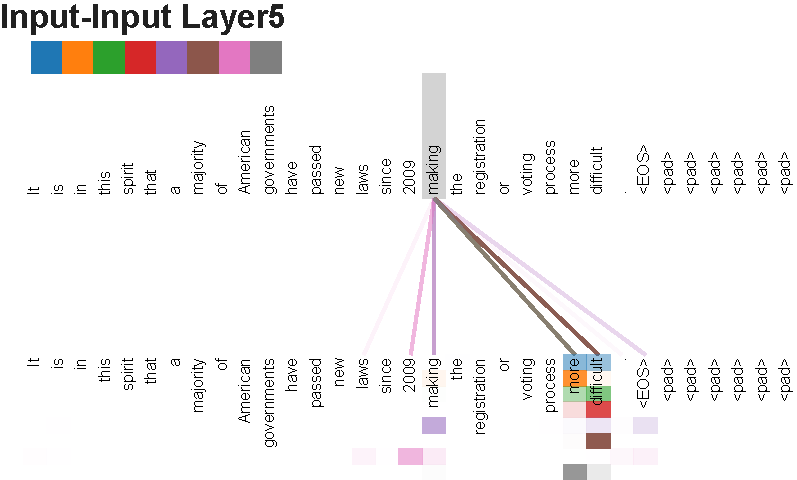
\includegraphics[width=\textwidth, trim=0 0 0 36, clip]{./vis/making_more_difficult5_new.pdf}}
\caption{一个展示编码器自注意力机制(第 5 层,共 6 层)中长距离依赖关系的注意力示例。许多注意力头关注动词 "making" 的远距离依赖,完成了短语 "making...more difficult"。此处仅展示单词 "making" 的注意力。不同颜色代表不同的注意力头。建议彩色查看。}
\end{figure*}

\begin{figure*}
{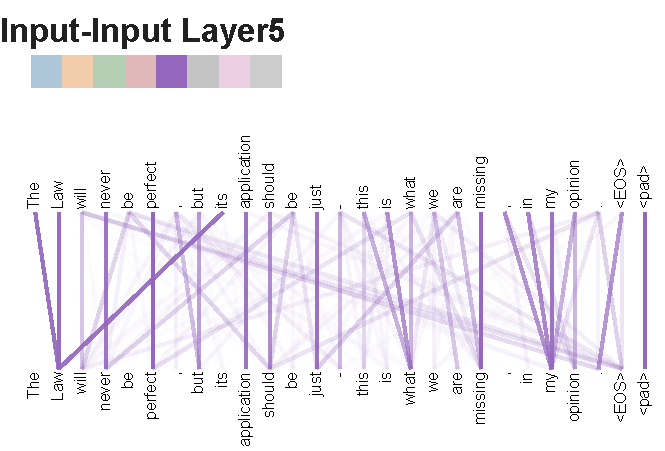
\includegraphics[width=\textwidth, trim=0 0 0 45, clip]{./vis/anaphora_resolution_new.pdf}}
{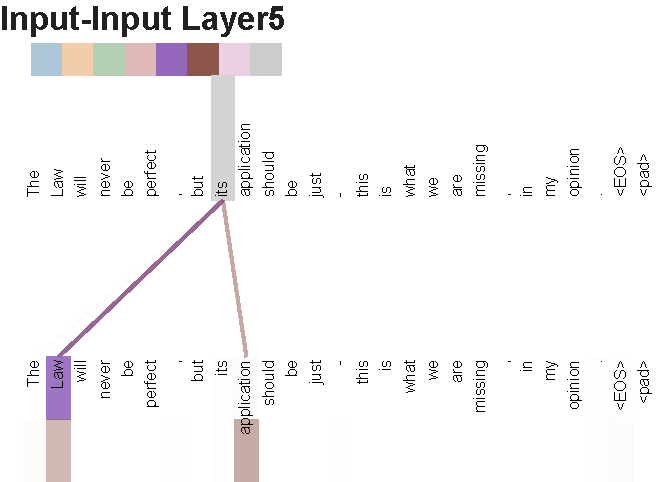
\includegraphics[width=\textwidth, trim=0 0 0 37, clip]{./vis/anaphora_resolution2_new.pdf}}
\caption{同样位于第 5 层(共 6 层)的两个注意力头,明显参与了 anaphora resolution(指代消解)。上图:头 5 的完整注意力。下图:仅针对单词 "its" 在头 5 和头 6 上的注意力隔离视图。注意该词的注意力分布非常集中。}
\end{figure*}

\begin{figure*}
{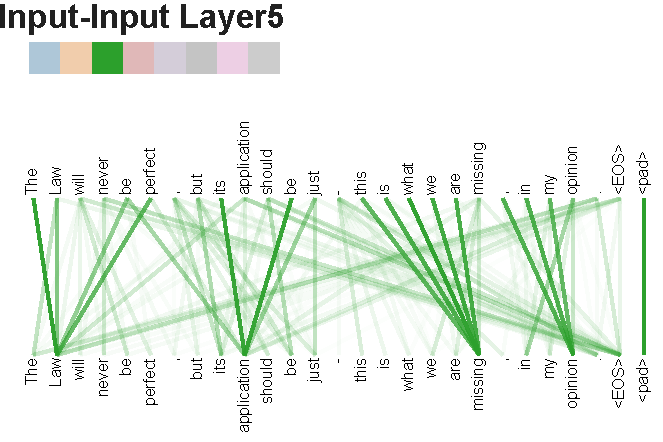
\includegraphics[width=\textwidth, trim=0 0 0 36, clip]{./vis/attending_to_head_new.pdf}}
{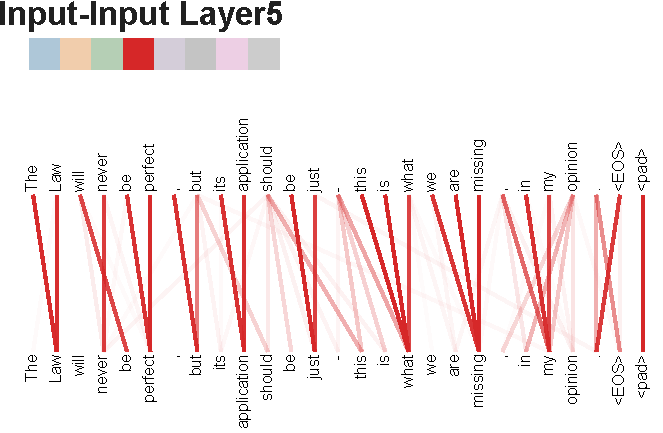
\includegraphics[width=\textwidth, trim=0 0 0 36, clip]{./vis/attending_to_head2_new.pdf}}
\caption{许多注意力头表现出与句子结构相关的行为模式。我们展示了来自编码器自注意力第 5 层(共 6 层)的两个不同头的两个此类示例。这些注意力头明显学会了执行不同的任务。}
\end{figure*}

%\appendix
%\newpage
%\pagebreak
\section*{两个前馈层 = 参数注意力}\label{sec:parameter_attention}

除了注意力层之外,我们的模型还包含逐位置前馈网络(第 \ref{sec:ffn} 节),该网络由两个线性变换组成,中间有一个 ReLU 激活函数。事实上,这些网络也可以被视为一种注意力形式。比较此类网络的公式与简单点积注意力层的公式(偏置和缩放因子已省略):

\begin{align*}
    FFN(x, W_1, W_2) = ReLU(xW_1)W_2 \\
    A(q, K, V) = Softmax(qK^T)V
\end{align*}

基于这些公式的相似性,两层前馈网络可以看作是一种注意力,其中键和值是可训练参数矩阵 $W_1$ 和 $W_2$ 的行,并且我们在兼容性函数中使用 ReLU 代替 Softmax。

%兼容性函数是 $compat(q, k_i) = ReLU(q \cdot k_i)$ 而不是 $Softmax(qK^T)_i$。

基于这种相似性,我们尝试用注意力层替换逐位置前馈网络,这些注意力层类似于我们模型中其他地方使用的层。多头参数注意力子层与 \ref{sec:multihead} 节中描述的多头注意力相同,不同之处在于每个注意力头的“键”和“值”输入是可训练模型参数,而不是前一层的线性投影。这些参数按比例放大 $\sqrt{d_{model}}$ 倍,以更类似于激活值。

在第一个实验中,我们将每个逐位置前馈网络替换为一个多头参数注意力子层,该子层有 $h_p=8$ 个头,键维度 $d_{pk}=64$,值维度 $d_{pv}=64$,每个注意力头使用 $n_p=1536$ 个键值对。该子层总共有 $2097152$ 个参数,包括查询投影和输出投影中的参数。这与我们替换的逐位置前馈网络中的参数数量匹配。虽然理论计算量也相同,但在实践中,注意力版本导致步长时间增加了约 $30\%$。

在第二个实验中,我们使用 $h_p=8$ 个头,每个注意力头有 $n_p=512$ 个键值对,再次匹配基础模型中的参数总数。第一个实验的结果略差于基础模型,第二个实验的结果略好于基础模型,参见表~\ref{tab:parameter_attention}。

\begin{table}[h]
\caption{用多头参数注意力替换逐位置前馈网络产生了与基础模型相似的结果。所有指标均在英德翻译开发集 newstest2013 上。}
\label{tab:parameter_attention}
\begin{center}
\vspace{-2mm}
%\scalebox{1.0}{
\begin{tabular}{c|cccccc|cccc}
\hline\rule{0pt}{2.0ex}
 & \multirow{2}{*}{$\dmodel$} & \multirow{2}{*}{$\dff$} &
\multirow{2}{*}{$h_p$} & \multirow{2}{*}{$d_{pk}$} & \multirow{2}{*}{$d_{pv}$} &
 \multirow{2}{*}{$n_p$} &
 PPL & BLEU & params & training\\
 & & & & & &  & (dev) & (dev) & $\times10^6$ & time \\
\hline\rule{0pt}{2.0ex}
base & 512 & 2048 & & & & & 4.92 & 25.8 & 65 & 12 hours\\
\hline\rule{0pt}{2.0ex}
AOP$_1$ & 512 & & 8 & 64 & 64 & 1536 & 4.92& 25.5  & 65 & 16 hours\\
AOP$_2$ & 512 & & 16 & 64 & 64 & 512 & \textbf{4.86} & \textbf{25.9}  & 65 & 16 hours \\
\hline
\end{tabular}
%}
\end{center}
\end{table}


%\section*{点积注意力中缩放因子的理由}

在第~\ref{sec:scaled-dot-prod}节中,我们介绍了缩放点积注意力,其中我们将点积按 $\sqrt{d_k}$ 缩放。在本节中,我们将给出这个缩放因子的大致理由。如果我们假设 $q$ 和 $k$ 是 $d_k$ 维向量,其分量是均值为 $0$、方差为 $1$ 的独立随机变量,那么它们的点积 $q \cdot k = \sum_{i=1}^{d_k} u_iv_i$ 的均值为 $0$,方差为 $d_k$。由于我们希望这些值的方差为 $1$,因此我们除以 $\sqrt{d_k}$。

%对于任意两个 $d_k$ 维向量 $\vec{u}$ 和 $\vec{v}$,其维度是独立的,点积的均值和方差将是各维度均值和方差乘积的求和,即 $E[<\vec{u},\vec{v}>] = \sum_{i=1}^{d_k} E[u_i]E[v_i]$,且 $E[(<\vec{u},\vec{v}>-E[<\vec{u},\vec{v}>])^2] = \sum_{i=1}^{d_k} E[({u_i}-E[u_i])^2] E[({v_i}-E[v_i])^2]$。层归一化鼓励每个维度的均值和方差分别为 $0$ 和 $1$,从而导致点积的均值分别为 $0$ 和 $d_k$。因此,按 $\sqrt{d_k}$ 缩放鼓励 logits 也被归一化。

\iffalse

在本节中,我们将给出这个缩放因子的大致理由,即我们将证明对于任意两个向量 $\vec{u}$ 和 $\vec{v}$,其方差和均值分别为 $1$ 和 $0$,点积的方差和均值分别为 $d_k$ 和 $0$。因此,除以 $\sqrt{d_k}$ 确保注意力 logits 的每个分量都被归一化。每个 Transformer 层中的重复层归一化鼓励 $\vec{u}$ 和 $\vec{v}$ 被归一化。

\begin{align*}
    E[<\vec{u},\vec{v}>] & =  \sum_k E[u_i v_i] &\text{由期望的线性性} \\
    & =\sum_k E[u_i]E[v_i] & \text{假设独立性} \\
    & = 0
\end{align*}

\begin{align*}
    E[(<\vec{u},\vec{v}>-E[<\vec{u},\vec{v}>])^2]  & = E[(<\vec{u},\vec{v}>)^2] - E[<\vec{u},\vec{v}>]^2 \\
    & = E[(<\vec{u},\vec{v}>)^2] \\
    & =  \sum_k E[{u_i}^2] E[{v_i}^2] &\text{由期望的线性性和独立性} \\
    & = d_k
\end{align*}

\fi


\end{document}
